\chapter{可視化システム}
\label{chap:system}
\cref{chap:access}からアクセス環境によってスループットに差が生じることがわかった.しかし,アクセス環境の影響についてユーザーに伝えているスピードテストサイトがない.そこで,本章ではアクセス環境の影響をユーザーに伝えるための可視化システム,iNoniusスピードテスト統計情報可視化システムについて述べる.

\section{システムの概要}
\subsection{システムの構成}
\cref{fig:system_image} にシステム構成を示す.システムは,iNonius統計情報可視化システムサーバーとiNonius Speed Testサーバー,クライアント端末から構成される.iNonius統計情報可視化システムサーバーには,Webサーバーコンテナと画像生成コンテナ,データ処理コンテナ,可視化システム用DBが存在する.データ処理コンテナはiNonius スピードテストサーバーから毎月の計測ログを取得し,アクセス環境ごとに最大値,最小値,中央値,四分位範囲,平均値からなる統計情報を算出し,統計量記録用テーブルに保存する.統計量記録用テーブルから 1 年分の統計量を取得して,表示用の画像を作成して,グラフ画像記録用テーブルにバイナリデータとして保存する.クライアントからのアクセス環境ごとの集計結果の要求を Web サーバーコンテナを受け取ると画像生成コンテナを経由して,グラフ画像記録用テーブルからバイナリデータを取得後,要求に対応する 1 年分の集計結果のグラフを画像(JPEG) ファイルとしてクライアントに返す.\cref{fig:system_v6_catv_dl}はアクセス回線が CATV の場合の IPv6 のダウンロードスループットのグラフである.可視化サイトにはアクセス環境ごとに IPv4 と IPv6,ダウンロードとアップロードのスループットをそれぞれ示す 4 つのグラフが表示される.

%\begin{comment}
\begin{figure}[htbp]
    \centering
    \vspace{40pt} % Adjust the space between the figures
    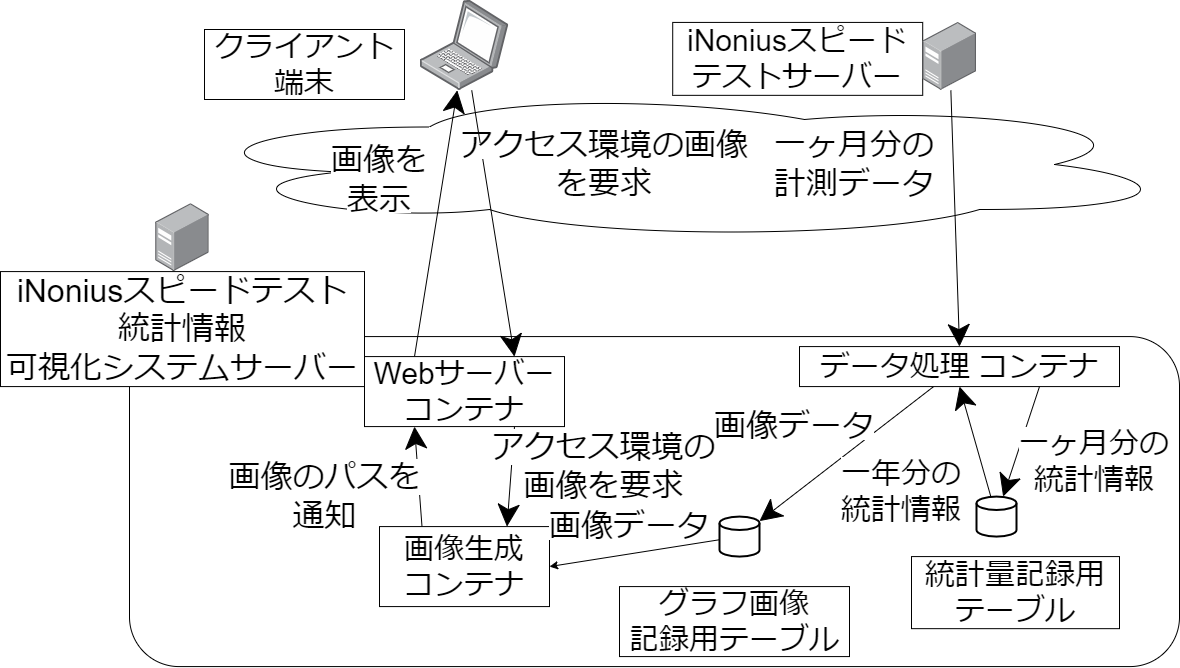
\includegraphics[width=1.0\textwidth]{fig/system_image.png}
    \caption{iNonius スピードテストサイト統計情報可視化システムのシステム構成}
    \label{fig:system_image}
    \vspace{20pt} % Adjust the space between the figures
    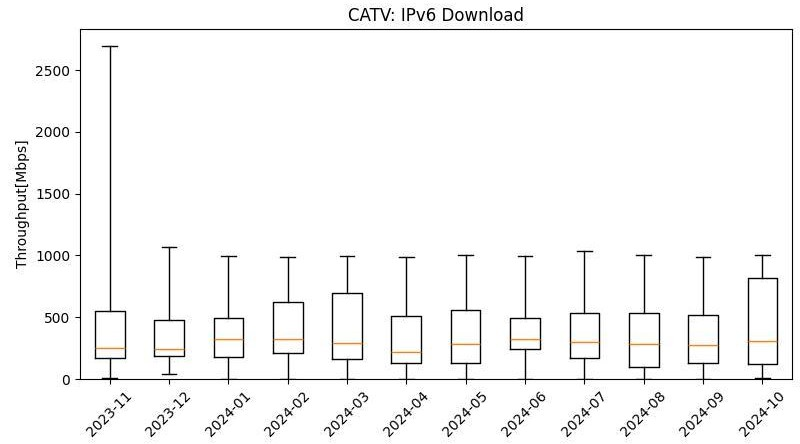
\includegraphics[width=1.0\textwidth]{fig/box_image.jpg}
    \caption{CATV回線のダウンロード速度のグラフ}
    \label{fig:system_v6_catv_dl}
    \vspace{40pt} % Adjust the space between the figures
\end{figure}
\FloatBarrier
%\end{comment}

\subsection{データ処理コンテナ}
データ処理コンテナ内で実行されるデータ処理とグラフ画像の作成フローを\cref{fig:graph_flow}に示す.iNonius Speed Testのデータベースから毎月の計測ログを取得し,前処理として外れ値を含む計測ログを除外する.このとき,外れ値として除外されるのは欠損値を含むデータとスループットの計測結果が小数第2位まで0を記録するデータである.欠損値を含むデータは統計情報を算出するときに,エラーの原因になるため除外する.スループットの計測結果が小数第2位まで0を記録するデータは計測が完了していない不完全なデータと推定されるため,異常値として除外している.アクセス環境の分類は,\cref{label:accesstype}と同様の手法を用いて分類している.アクセス環境ごとに最大値,最小値,中央値,四分位範囲,平均値からなる統計情報を算出し統計量記録用テーブルを更新する.統計量記録用テーブルには,アクセス環境の種類とデータの期間,アップロードとダウロードの判定フラグ,IPv4/IPv6の判定フラグ,統計情報が記録される.統計量記録用テーブルから 1 年分の統計量を取得して\cref{fig:system_v6_catv_dl}のような表示用のグラフ画像を作成する.グラフには箱ひげ図を用いている.箱ひげ図を用いることで,計測ログの分布を可視化できることを目的としている.また,総務省が発表している通信品質の調査に関するガイドライン\cite{mobile_guideline}\cite{bb_guideline}でも採用されており,通信品質を可視化するのに適していると考えられる.画像のバイナリデータをグラフ画像記録用テーブルにアクセス環境の種類とデータの期間,アップロードとダウロードの判定フラグ,IPv4/IPv6の判定フラグとともに保存する.
一連の処理を月次で実行しているため,毎月の計測ログから統計情報を算出し,グラフ画像を作成している.

%\begin{comment}
\begin{figure}[htbp]
    \centering
    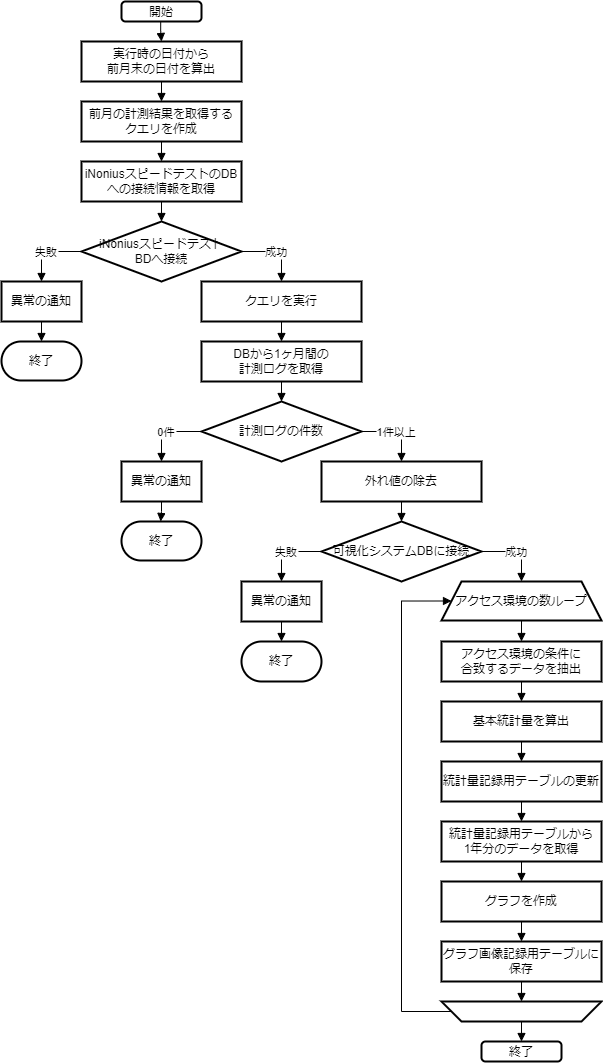
\includegraphics[width=0.8\textwidth]{fig/graph_flow.png}
    \caption{データ処理コンテナの処理フロー}
    \label{fig:graph_flow}
\end{figure}
\FloatBarrier
%\end{comment}

\subsection{画像生成コンテナ}
画像生成コンテナはクライアントからのアクセス環境ごとの集計結果の要求を受け取り,グラフ画像記録用テーブルからバイナリデータを取得して,要求に対応する 1 年分の集計結果のグラフを画像(JPEG)ファイルとしてクライアントに返すコンテナである.Webサーバーコンテナと画像生成コンテナの処理フローをそれぞれ\cref{fig:web_flow},\cref{fig:fig_flow}に,シーケンス図を\cref{fig:sequence}に示す.
Webサーバーコンテナはクライアントからのリクエストを受け取り,画像生成コンテナにアクセス環境に基づいたグラフ画像の生成をリクエストする.画像生成コンテナはグラフ画像記録用テーブルから必要なデータを取得し,グラフ画像を生成して一時ファイルとしてホスト上に保存する.その後,Webサーバーコンテナに一時ファイルのアドレスを返し,Webサーバーコンテナはクライアントにグラフ画像を表示する.

%\begin{comment}
\begin{figure}[htbp]
    \centering
    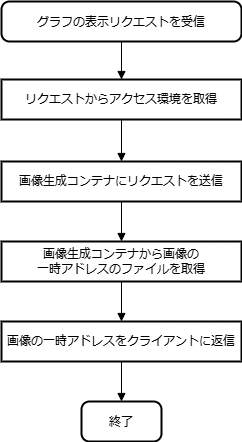
\includegraphics[width=0.6\textwidth]{fig/web_flow.png}
    \caption{Webサーバーコンテナの処理フロー}
    \label{fig:web_flow}
\end{figure}
\FloatBarrier
%\end{comment}

%\begin{comment}
\begin{figure}[htbp]
    \centering
    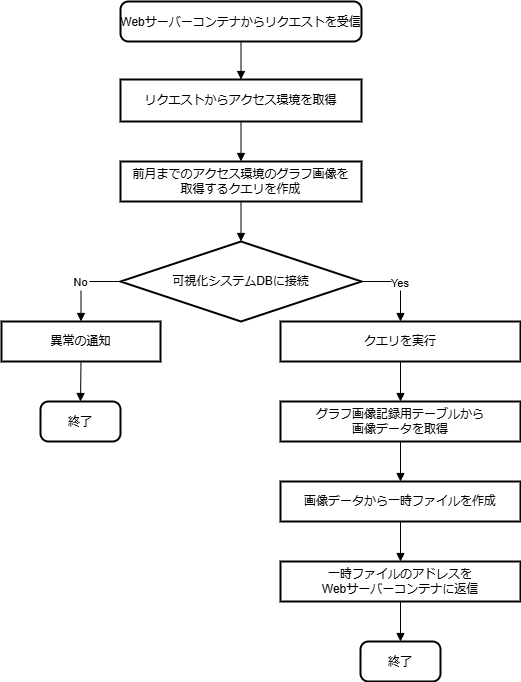
\includegraphics[width=1.0\textwidth]{fig/fig_flow.png}
    \caption{画像生成コンテナの処理フロー}
    \label{fig:fig_flow}
\end{figure}
\FloatBarrier
%\end{comment}

%\begin{comment}
\begin{figure}[htbp]
    \centering
    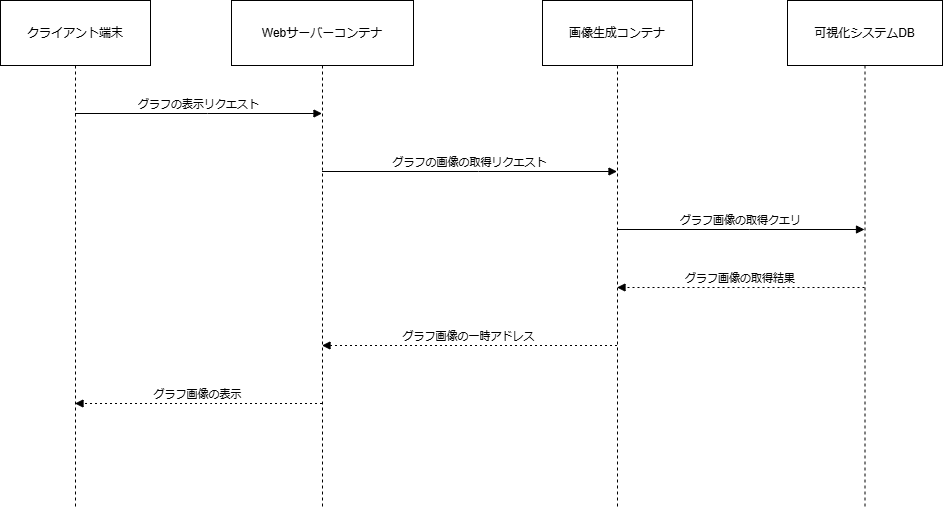
\includegraphics[width=1.0\textwidth]{fig/sequence.png}
    \caption{シーケンス図}
    \label{fig:sequence}
\end{figure}
\FloatBarrier
%\end{comment}

\subsection{開発環境}
開発システムのホストの開発環境を\cref{tab:host}に,Webサーバーコンテナの開発環境を\cref{tab:webserver}に,画像生成コンテナの開発環境を\cref{tab:image}に,データ処理コンテナの開発環境を\cref{tab:dataprocessing}に,データベースコンテナの開発環境を\cref{tab:database}に示す.

\begin{table}
    \centering
    \caption{ホストの開発環境}
    \label{tab:host}
    \begin{tabular}{cc}
        \hline
        項目 & 説明 \\
        \hline \hline
        OS & Ubuntu Ubuntu 22.04.5 LTS \\
        カーネル & 5.15.0-125-generic \\
        CPU & Inter(R) Core(TM) i7-9700 CPU @ 3.00GHz \\
        メモリ & 15GB \\
        Docker & Docker version 27.2.0, build 3ab4256 \\
        \hline
    \end{tabular}
\end{table}

\begin{table}
    \centering
    \caption{Webサーバーコンテナの開発環境}
    \label{tab:webserver}
    \begin{tabular}{cc}
        \hline
        項目 & 説明 \\
        \hline \hline
        OS & Alpine Linux v3.20 \\
        \hline
        nginx & nginx/1.27.2 \\
        \hline
        \end{tabular}
\end{table}

\begin{table}
    \centering
    \caption{画像生成コンテナの開発環境}
    \label{tab:image}
    \begin{tabular}{cc}
        \hline
        項目 & 説明 \\
        \hline \hline
        OS & Debian GNU/Linux 12 (bookworm) \\
        \hline
        Python & Python 3.9.20 \\
        \hline
        Flask & 3.0.3 \\
        \hline
        Flask-Cors & 5.0.0 \\
        \hline
        PyMySQL & 1.1.1 \\
        \hline
        SQLAlchemy & 2.0.36 \\
        \hline
    \end{tabular}
\end{table}

\begin{table}
    \centering
    \caption{データ処理コンテナの開発環境}
    \label{tab:dataprocessing}
    \begin{tabular}{cc}
        \hline
        項目 & 説明 \\
        \hline \hline
        OS & Debian GNU/Linux 12 (bookworm) \\
        \hline
        Python & Python 3.9.20 \\
        \hline
        PyMySQL & 1.1.1 \\
        \hline
        SQLAlchemy & 2.0.36 \\
        \hline
        matplotlib & 3.9.2 \\
        \hline
        numpy & 2.1.2 \\
        \hline
        pandas & 2.2.3 \\
        \hline
    \end{tabular}
\end{table}

\begin{table}
    \centering
    \caption{データベースコンテナの開発環境}
    \label{tab:database}
    \begin{tabular}{cc}
        \hline
        項目 & 説明 \\
        \hline \hline
        OS & Ubuntu 24.04.1 LTS \\
        \hline
        MariaDB & mariadb from 11.5.2-MariaDB \\
        \hline
        \end{tabular}
\end{table}

\section{システムの評価}
\subsection{ユーザーアンケート}
本システムはWebサイトとして\url{https://inonius.v6.netsci.info.hiroshima-cu.ac.jp/}で公開している.このサイトを利用したユーザーにアンケートを実施したアンケートをもとに評価を行う.
アンケートの設問を\cref{tab:questionnaire}に示す.設問は全部で 10 問あり,そのうちQ1からQ4は,本サイトを利用してもらうための質問であるため,それらは評価から除外してQ5からQ10について評価を行う.
Q5からQ7の回答を\cref{fig:Q5}から\ref{fig:Q7}に示す.
%\cref{tab:questionnaire}

\begin{table}[htbp]
    \centering
    \caption{アンケート項目}
    \begin{tabular}{lll}
        \hline
        番号 & 質問 & 回答方法 \\
        \hline \hline
        \vspace{10pt}
        Q1.&
        \begin{tabular}{l}
            普段,インターネットを使用しているときの\\通信品質の満足度をお答えください.\\
        \end{tabular}& 5段階評価\\
        \vspace{10pt}
        Q2.&
        \begin{tabular}{l}
            普段のインターネットを使用しているときの\\体感の通信品質と,iNoniusスピードテストの\\計測結果を比較したときどちらが上回っていますか?\\
        \end{tabular}& 5段階評価\\
        \vspace{10pt}
        Q3-1.&
        \begin{tabular}{l}
            本サイトの統計情報のうちあなたと同じアクセス環境の\\統計情報の直近1カ月の中央値とiNoniusスピードテストでの\\計測結果を直近比較したとき,どちらが速いですか?\\
        \end{tabular}& 5段階評価\\
        \vspace{10pt}
        Q3-2.&
        \begin{tabular}{l}
            本サイトの統計情報のうちあなたと異なるアクセス環境の\\統計情報の直近1カ月の中央値ととiNoniusスピードテストでの\\計測結果を直近比較したとき,どちらが速いですか?\\
        \end{tabular}& 5段階評価\\
        \vspace{10pt}
        Q4.&
        \begin{tabular}{l}
            本サイトの統計情報とiNoniusスピードテストの計測結果を\\比較して,ご自身の通信環境を見直そうと思いましたか?\\
        \end{tabular}& 4段階評価\\
        \vspace{10pt}
        Q5.&
        \begin{tabular}{l}
            iNoniusスピードテストの統計情報を可視化できることに\\意義を感じますか.\\
        \end{tabular}& 5段階評価\\
        \vspace{10pt}
        Q6.&
        \begin{tabular}{l}
            アクセス環境別の統計情報と計測結果を比較することに\\意義を感じたか.\\
        \end{tabular}& 5段階評価\\
        \vspace{10pt}
        Q7.&
        \begin{tabular}{l}
            本サイトで使用しているグラフ(箱ひげ図)の表現は\\適切だと思いますか.\\
        \end{tabular}& 5段階評価\\
        \vspace{10pt}
        Q8.&
        \begin{tabular}{l}
            上記の質問で「そう思わない」,「あまりそう思わない」と\\回答された方は,なぜそう思われたか,また改善案を\\教えてください.\\
        \end{tabular}& 自由記述\\
        \vspace{10pt}
        Q9.&
        \begin{tabular}{l}
            現在,アクセス環境によるスピードテストサイトでの\\計測に対する影響は調査を続けております.\\本サイトで定義しているアクセス環境以外に,\\調査してほしい条件などありましたらご意見ください.\\
        \end{tabular}& 自由記述\\
        \vspace{10pt}
        Q10.&
        \begin{tabular}{l}
            その他に本サイト並びに研究について自由にご意見ください.\\
        \end{tabular}& 自由記述\\
        \hline
    \end{tabular}
    \label{tab:questionnaire}
\end{table}
\FloatBarrier

Q5の回答から統計情報を可視化することは多くのユーザーが肯定来な回答をしているため,必要とされていることがわかる.一方で,Q6の回答からアクセス環境別の統計情報と計測結果を比較することに意義を感じるユーザーは全体の約70\%とQ5に比べて少ない.Q9で本サイトで示しているアクセス環境以外に調査してほしいアクセス環境を尋ねたところ,アクセス網の利用用途による違い,地理的な違い,アクセス網の種類を増やすことなどが挙げられた.公開したシステムではユーザーが知りたいようなアクセス環境を示すことができていないため,肯定的な意見が少ないと考えられる.定義しているアクセス環境は計測ログに含まれる情報から選択しているため,ユーザーが知りたいアクセス環境を示すことができていない.今後はさまざまな情報を計測ログに付与してユーザーに必要とされるアクセス環境を示すことができるようにする必要がある.

Q7のグラフの表現についても肯定的な意見が全体の約70\%である.Q7で「あまりそう思わない」「そう思わない」と回答したユーザーにQ8でなぜそう思ったかを自由記述で尋ねた.グラフのスケールの調整ができず比較が難しい,データの分布に関する情報が欲しい,という意見が挙がっている.本システムではグラフは画像で表示しているため,ユーザーはインタラクティブにグラフを操作することができず,比較が難しい.\cref{fig:bad_boxplot}に箱ひげ図の例を示す.この図はFTTH回線のダウンロード速度の箱ひげ図である.この図の,2023-12と2024-01の箱ひげ図は最小値と中央値,第1四分位数が重なっているように見えるため,比較することが難しい場合が考えられる.データの分布に関しては,箱ひげ図は第1四分位数,中央値,第3四分位数,最小値,最大値を表現しているため,データの分布に関する情報が得られると考えていたが,箱ひげ図はデータの分布を正確に表現することが難しい.スループットの計測結果は正規分布ではないため,データのボリューム層がどこにあるかを知るためには他の情報も必要である.今後はユーザーがインタラクティブにグラフを操作できるようにすることで,比較が容易になるようにする必要がある.また,データの分布に関する情報を示すために他のグラフを併用することで,データの分布に関する情報を得やすくする必要がある.これらを実現すること,アクセス環境の違いをよりわかりやすく示すことが今後の課題である.

%\begin{comment}
\begin{figure}[htbp]
    \centering
    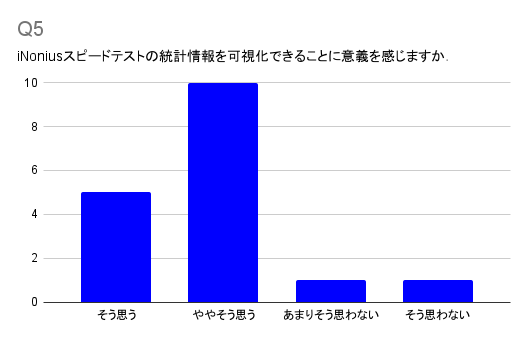
\includegraphics[width=1.0\textwidth]{fig/Q5.png}
    \caption{Q5のアンケート結果}
    \label{fig:Q5}

    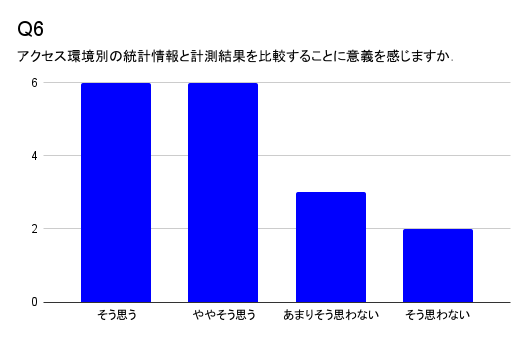
\includegraphics[width=1.0\textwidth]{fig/Q6.png}
    \caption{Q6のアンケート結果}
    \label{fig:Q6}
\end{figure}
\FloatBarrier

\begin{figure}[htbp]
    \centering
    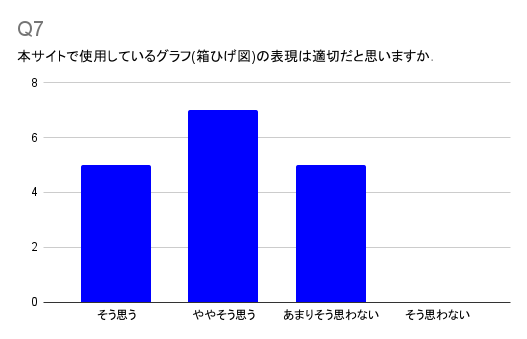
\includegraphics[width=1.0\textwidth]{fig/Q7.png}
    \caption{Q7のアンケート結果}
    \label{fig:Q7}
\end{figure}
\FloatBarrier
%\end{comment}

%\begin{comment}
\begin{figure}[htbp]
    \centering
    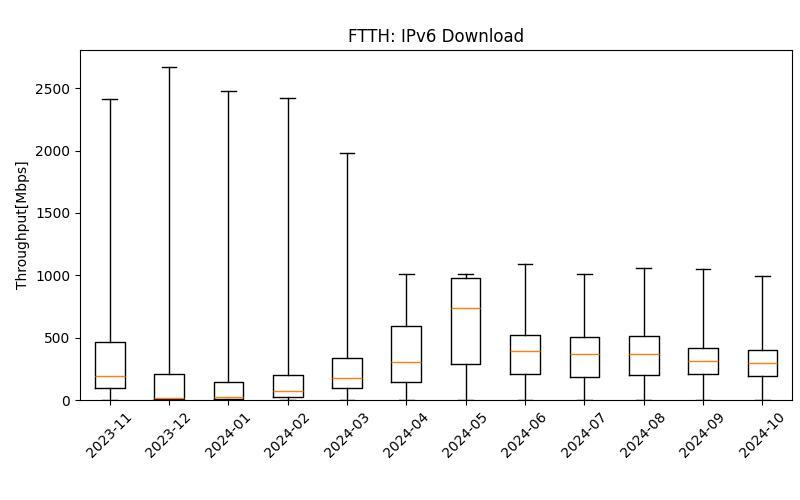
\includegraphics[width=1.0\textwidth]{fig/system_v6_ftth_dl.jpg}
    \caption{FTTH回線のダウンロード速度の箱ひげ図}
    \label{fig:bad_boxplot}
\end{figure}
\FloatBarrier
%\end{comment}

\subsection{類似するサービスとの比較}
スピードテストサイトは多く運用されており,その中には統計情報を提供しているサイトとして,みんなのネット回線速度\cite{minsoku}とRadish Network Speed Testing\cite{radish}が挙げられる.これらのサイトと本システムを比較して評価する.

みんなのネット回線速度でもアクセス網の種類やISPごとに平均値とランキング形式で公開している.また個々の計測結果も公開されており,その計測が行われたアクセス環境も併せて公開されている.しかしグラフなどによるデータの分布に関する情報は提供されていないため,それぞれの結果がどのような分布になっているかを知ることができない.そのため自分の環境と比較してどの程度のスループットが得られるかを知ることが難しい.本システムと比較すると,個別の計測結果の詳細は公開していないが,箱ひげ図を用いたアクセス環境ごとの統計情報を提供しているため,データの分布に関する情報を得やすいと言える.

Radish Network Speed Testingは計測ログの統計を四半期ごとに公開しており,全体のデータだけでなくアクセス網の種類やISPごとにデータを提供している.ISP毎の情報では提供しているサービス別でも提供しているため,ユーザーが知りたい情報を提供している.使用されているグラフは2種類の棒グラフを組み合わせて使用している.片方の棒グラフにはパーセントタイルを色分けして表現しており,もう一つの棒グラフには色の濃淡で分布強度を示している.2つのグラフを組み合わせることで,ユーザーはデータの分布に関する情報を得やすい.またスループットのスケールを100Mbpsまでのグラフと1Gbpsのグラフの2つを用意している.本システムと同様にグラフを画像で提供しているが,ユーザーがスケールの調整ができるように工夫がされている.しかし,このサイトで行われるISPやサービスの判定はユーザーからの入力によるものであるため,正確な情報を提供することが難しいことが課題として考えられる.また,グラフが1Gbpsまでしか描画されない.本研究で使用している計測ログには1Gbps以上のスループットを示す含まれていることから,対応できるようにする必要がある.これらの課題に対しては本システムで解決している.また,計測のサービスは現在でも稼働しているが,統計情報の更新は2013年以降更新されていない.

以上の類似サービスと比較したとき,本システムは必要な統計情報を提供しているため,ユーザーにとって有用であると言える.また現代のスループットに併せたスケールに調整したグラフで表示しているため,ユーザーがスループットの比較を行いやすいと言える.しかし見せ方に関してはRadish Network Speed Testingのように多角的な情報を提供できておらず,改善の予知があるといえる.また表示できるアクセス環境の種類や詳細な情報に関しては,本システムの方が不足している部分が多く,今後の課題として考えられる.

\section{まとめ}
本章では,アクセス環境によるスループットへの影響をユーザーに可視化するシステムについて述べた.アンケートの結果から統計情報の可視化に対して肯定的な意見が得られた一方で,アクセス環境ごとの可視化については肯定的な意見が少なかった.類似サービスと比較したときに表示できるアクセス環境の種類が少なく,ユーザーが期待している情報が表示できていない可能性が考えられる.今後はユーザーが知りたい情報を提供できるようにするために,通信品質への影響についてさらに調査をする必要ある.またグラフの表示に関しても,スケールの調整などインタラクティブな操作ができるようにすることで,ユーザーがデータの分布に関する情報を得やすくする必要がある.